\documentclass[a4paper,10pt, notitlepage]{report}
\usepackage{geometry}
\geometry{verbose,tmargin=30mm,bmargin=25mm,lmargin=25mm,rmargin=25mm}
\usepackage[utf8]{inputenc}
\usepackage[sectionbib]{natbib}
\usepackage{amssymb}
\usepackage{amsmath}
\usepackage{bbm}
\usepackage{enumitem}
\usepackage{xcolor}
\usepackage{cancel}
\usepackage{mathtools}
\usepackage{cancel}
\usepackage{caption}
\usepackage{subcaption}
\usepackage{float}
\usepackage{lipsum}
\PassOptionsToPackage{hyphens}{url}\usepackage{hyperref}
\hypersetup{colorlinks=true,citecolor=blue}

\newtheorem{thm}{Theorem}
\newtheorem{lemma}[thm]{Lemma}
\newtheorem{proposition}[thm]{Proposition}
\newtheorem{remark}[thm]{Remark}
\newtheorem{defn}[thm]{Definition}

\newcommand{\ind}{\hspace{6mm}}

%%%%%%%%%%%%%%%%%%%% Notation stuff
\newcommand{\pr}{\operatorname{Pr}} %% probability
\newcommand{\vr}{\operatorname{Var}} %% variance
\newcommand{\ev}{\mathbb{E}}
\newcommand{\Bin}{\operatorname{Binomial}}
\newcommand{\Poi}{\operatorname{Poisson}}
\newcommand{\Geom}{\operatorname{Geometric}}
\newcommand{\DGamma}{\operatorname{Gamma}}
\newcommand{\Beta}{\operatorname{Beta}}
\newcommand{\Normal}{\operatorname{Normal}}
\newcommand{\logit}{\operatorname{logit}}
\newcommand{\one}{\mathbbm{1}}


\newcommand{\rs}{X_1, X_2, \ldots, X_n} %%  random sample
\newcommand{\irs}{X_1, X_2, \ldots} %% infinite random sample
\newcommand{\rsd}{x_1, x_2, \ldots, x_n} %%  random sample, realized
\newcommand{\bX}{\boldsymbol{X}} %%  random sample, contracted form (bold)
\newcommand{\bx}{\boldsymbol{x}} %%  random sample, realized, contracted form (bold)
\newcommand{\bT}{\boldsymbol{T}} %%  Statistic, vector form (bold)
\newcommand{\bt}{\boldsymbol{t}} %%  Statistic, realized, vector form (bold)
\newcommand{\emv}{\hat{\theta}}
\DeclarePairedDelimiter\ceil{\lceil}{\rceil}
\DeclarePairedDelimiter\floor{\lfloor}{\rfloor}

% Title Page
\title{Exam 2 (A2)}
\author{Class: Bayesian Statistics \\ Instructor: Luiz Max Carvalho}
\date{02/06/2021}

\begin{document}
\maketitle

\textbf{Turn in date: until 09/06/2021 at 23:59h Brasilia Time.}

\begin{center}
\fbox{\fbox{\parbox{0.9\textwidth}{\textsf{
    \begin{itemize}
    \item Please read through the whole exam before starting to answer;
    \item State and prove all non-trivial mathematical results necessary to substantiate your arguments;
    \item Do not forget to add appropriate scholarly references~\textit{at the end} of the document;
    \item Mathematical expressions also receive punctuation;
    \item You can write your answer to a question as a point-by-point response or in ``essay'' form, your call;
    \item Please hand in a single, \textbf{typeset} ( \LaTeX) PDF file as your final main document.
 Code appendices are welcome,~\textit{in addition} to the main PDF document.
    \item You may consult any sources, provided you cite \textbf{ALL} of your sources (books, papers, blog posts, videos);
    \item You may use symbolic algebra programs such as Sympy or Wolfram Alpha to help you get through the hairier calculations, provided you cite the tools you have used.
    \item The exam is worth 100 %$\min\left\{\text{your\:score}, 100\right\}$
    marks.
    \end{itemize}}
}}}
\end{center}

\newpage

\section*{Background}

This exam covers applications, namely estimation, prior sensitivity and prediction.
You will need a working knowledge of basic computing tools, and knowledge of MCMC is highly valuable.
Chapter 6 in \cite{Robert2007} gives an overview of computational techniques for Bayesian statistics.

\section*{Inferring population sizes -- theory}

Consider the model
\begin{equation*}
 x_i \sim \operatorname{Binomial}(N, \theta),
\end{equation*}
with \textbf{both} $N$ and $\theta$ unknown and suppose one observes $\boldsymbol{x} = \{x_1, x_2, \ldots, x_K\}$.
Here, we will write $\xi = (N, \theta)$.

\begin{enumerate}[label=\alph*)]
 \item (10 marks) Formulate a hierarchical prior ($\pi_1$) for $N$, i.e., elicit $F$ such that $N \mid \alpha \sim F(\alpha)$ and $\alpha  \sim \Pi_A$.
 Justify your choice; 

 \vspace{2ex}

\fbox{\parbox{0.92\textwidth}{
    {\bf Solution.} The only restriction prior to the data we have is that $N \in
    \mathbb{Z}^+$. Therefore we are looking for a distribution in this space.
    We can follow the assumption made by \cite{Raftery1988} where $N \sim
    \Poi(\mu)$. Other approach is to consider $N \sim \Geom(\nu)$.

    The first approach has the advantage in calculations. When 
    $$x_i | N, \theta \sim \Bin(N,\theta)$$ and $$N \sim \Poi(\mu),$$ we have that $x_i \sim
    \Poi(\mu\cdot\theta)$, as proved in Appendix \ref{sec:binomial-poisson}. And we can convert prior information in $x_i$ in
    terms of our beliefs about its mean. 

    The second approach serves as a comparative. The interesting part of this
    distribution is the compact domain since $\nu \in [0,1]$. From that, we
    can build a model that caries the correlation between $\nu$ and $\theta$
    whenever necessary in a direct way: we transform the variables to logistic
    space and defines a bivariate normal distribution. We would have to define
    five parameters, but this is a good extension. 

    \vspace{2ex}

    {\bf Priors to the hyperparameters}

    \vspace{2ex}

    Now we shall define the priors to the hyperparameters. Define $\lambda =
    \mu\cdot\theta$. Given that it is morel likely that previous research made
    statements about $x_i$, we use the same idea as Raftery considering the
    prior over $(\lambda, \theta)$. I will assume they are independent from
    now on with 
    $$
    \lambda \sim \DGamma(\alpha, \beta),
    $$
    and
    $$
    \theta \sim \Beta(a,b).
    $$

    The other approach will have two settings. First I suppose $\nu$ and
    $\theta$ independents with 
    $$
    \nu \sim \Beta(\alpha_1, \beta_1)
    $$
    and
    $$
    \theta \sim \Beta(\alpha_2, \beta_2).
    $$
    I choose the Beta distribution because it has a flexible shape with
    a good intuition behind it. Other point is that the Beta distribution
    forms a conjugate family for the Geometric distribution. Another set up is
    to consider the correlated case. We do it in the following way:
    $$
    \begin{pmatrix}
        \logit(\nu) \\ \logit(\theta) 
    \end{pmatrix} \sim \Normal(\eta, \Sigma).
    $$
}
}

\fbox{\parbox{0.92\textwidth}{
This choice is intrinsically linked to the fact the the normal distribution is
a good approximation to a series of events, and it has a very good
interpretation of the parameters. The problem with this approach is that it is
harder to codify prior information. We necessarily need information about $N$,
$\theta$, and how they relate. 

From these three approaches, I will call these approaches in the text (1)
{\em Raftery approach}, (2) {\em Geometric and independent approach}, and (3)
{\em Geometric
and correlated approach}. 

}}

\vspace{2ex}

 \item (5 marks) Using the prior from the previous item, write out the full joint posterior kernel for all unknown quantities in the model, $p(\xi \mid \boldsymbol{x})$. \textit{Hint:} do not forget to include the appropriate indicator functions!;
 
 \vspace{2ex}

\fbox{\parbox{0.92\textwidth}{
    {\bf Solution.} For the Geometric and correlated approach, it may be impossible to find a simple
    expression. 

    Generally speaking, by Bayes' Theorem, 
    \begin{equation}
    \label{eq:bayes-theorem}
    \begin{split}
        p(\xi|\bx) &\propto l(\xi|\bx)\cdot\pi(\xi) \\
        &= \left(\prod_{i=1}^n \binom{N}{x_i}\theta^{x_i}(1 - \theta)^{N-x_i}\one(N \ge x_i)\right)\cdot \pi(\xi) \\
        &= \left(\prod_{i=1}^n \binom{N}{x_i}\right)\theta^{S}(1 - \theta)^{nN - S}\cdot \pi(\xi)\cdot\one(N\ge x_{\max}), 
    \end{split}
    \end{equation}
    where $S = \sum_{i=1}^n x_i$. We shall derive for each case the prior
    $\pi(\xi)$. 

    \begin{enumerate}
        \item[(1)] {\bf Raftery}: 
        \begin{equation*}
            \begin{split}
                \pi(\xi) &= \int_0^{\infty} \pi(\xi, \lambda) \, d\lambda \\
                &= \int_0^{\infty} \pi(N|\theta,\lambda)\pi(\theta,\lambda) \, d\lambda \\
                &= \int_0^{\infty} \frac{e^{-\lambda/\theta}(\lambda/\theta)^{N}}{N!}\pi(\lambda)\pi(\theta) \, d\lambda\\
                &\propto  \int_0^{\infty} \frac{e^{-\lambda/\theta}(\lambda/\theta)^{N}}{N!}\lambda^{\alpha - 1}e^{-\beta \lambda}\theta^{a-1}(1-\theta)^{b-1}\one(0<\theta<1) \, d\lambda\\
                &= \frac{\theta^{a-1-N}(1-\theta)^{b-1}}{N!}\one(0<\theta<1)\int_0^{\infty} \lambda^{\alpha + N - 1}e^{-(\beta + 1/\theta)\lambda} \, d\lambda \\
                &= \frac{\theta^{a-1-N}(1-\theta)^{b-1}}{N!}\one(0<\theta<1)\cdot \frac{\Gamma(\alpha+N)}{(\beta + 1/\theta)^{\alpha + N}},
            \end{split}
        \end{equation*}
        since the integrand is the kernel of a gamma distribution. Therefore,
        rewriting,
        \begin{equation}
            \label{eq:prior-raftery}
            \pi(\xi) \propto \frac{\Gamma(\alpha+N)\theta^{a-1-N}(1-\theta)^{b-1}}{(\beta + 1/\theta)^{\alpha + N}N!}\one(0<\theta<1)
        \end{equation}
        and
        \begin{equation}
            \label{eq:posterior-raftery}
            p(\xi|\bx) \propto \left(\prod_{i=1}^n \binom{N}{x_i}\right)\frac{\Gamma(\alpha+N)\theta^{a+S-1-N}(1-\theta)^{b+nN-S-1}}{(\beta + 1/\theta)^{\alpha + N}N!}\one(0<\theta<1, N\ge x_{\max})
        \end{equation} 
    \end{enumerate}
}
}

\fbox{\parbox{0.92\textwidth}{

\begin{enumerate}

    \item[(2)] {\bf Geometric and independent}: 
        
    \begin{equation*}
        \begin{split}
            \pi(\xi) &= \int_0^{1} \pi(\xi, \nu) \, d\nu \\
            &= \int_0^{1} \pi(N|\nu,\theta)\pi(\nu)\pi(\theta) \, d\nu \\
            &\propto \theta^{\alpha_2-1}(1-\theta)^{\beta_2-1} \one(0<\theta<1) \int_0^{1} (1-\nu)^N\nu \cdot\nu^{\alpha_1 - 1}(1-\nu)^{\beta_1-1}\, d\nu \\
            &= \theta^{\alpha_2-1}(1-\theta)^{\beta_2-1} \one(0<\theta<1) \int_0^{1} \nu^{\alpha_1}(1-\nu)^{N+\beta_1-1}\, d\nu \\
            &= \theta^{\alpha_2-1}(1-\theta)^{\beta_2-1} \one(0<\theta<1) B(\alpha_1+1,N+\beta_1), 
        \end{split}
    \end{equation*}
    since the integrand is the kernel of a Beta distribution. Rewriting, 
    \begin{equation}
        \label{eq:prior-geom-iden}
        \pi(\xi) \propto B(\alpha_1+1,N+\beta_1)\theta^{\alpha_2-1}(1-\theta)^{\beta_2-1} \one(0<\theta<1) 
    \end{equation}
    and 
    \begin{equation}
        \label{eq:posterior-geom-iden}
        p(\xi|\bx) \propto \left(\prod_{i=1}^n \binom{N}{x_i}\right) B(\alpha_1+1,N+\beta_1)\theta^{S + \alpha_2-1}(1-\theta)^{nN + \beta_2-S-1} \one(0<\theta<1, N \ge x_{\max}) 
    \end{equation}

    \item[(3)]  {\bf Geometric and correlated}: This is the harder case. I
    have to derive $\pi(\nu,\theta)$ from $\pi(\logit(\nu), \logit(\theta))$.
    Define $f(x_1,x_2) = (\logit^{-1}(x_1), \logit^{-1}(x_2))$. This is an
    invertible function with $f^{-1}(y_1,y_2) = (\logit(y_1), \logit(y_2))$. By
    the change of variables, 
    $$
    \pi(\nu,\theta) = \pi(f^{-1}(\nu, \theta))\cdot\left|\det \left[\frac{df^{-1}(z)}{dz}\bigg|_{z=(\nu,\theta)}\right]\right|.
    $$
    Observe that 
    $$
    \det \left[\frac{df^{-1}(z)}{dz}\bigg|_{z=(\nu,\theta)}\right] = \det \begin{bmatrix}
        \frac{d}{d\nu}\logit(\nu) & 0 \\
        0 & \frac{d}{d\theta}\logit(\theta)
    \end{bmatrix} = \frac{d}{d\nu}\logit(\nu) \cdot \frac{d}{d\theta}\logit(\theta).
    $$
    By the calculation of the Jacobian, we can join everything
    \begin{equation*}
        \begin{split}
            \pi(\xi) &= \int_0^{1} \pi(N|\nu,\theta)\pi(\nu,\theta) \, d\nu  \\
            &= \int_0^1 (1-\nu)^N\nu \pi(\logit(\nu), \logit(\theta))|\logit '(\nu) \cdot \logit '(\theta)| \, d\nu \\
            &= \int_0^1 (1-\nu)^N\nu \pi(\logit(\nu), \logit(\theta))\frac{1}{\nu(1-\nu)\theta(1-\theta)}\, d\nu \\ 
            &= \frac{1}{\theta(1-\theta)}\int_0^1 (1-\nu)^{N-1}\pi(\logit(\nu), \logit(\theta)) \, d\nu . \\
        \end{split}
    \end{equation*} 
    Let $z = (\logit(\nu), \logit(\theta))$. Therefore, 
    \begin{equation}
        \label{eq:prior-geom-corr}
        \pi(\xi) \propto \frac{1}{\theta(1-\theta)}\int_0^1 (1-\nu)^{N-1}\exp\left\{-\frac{1}{2}(z - \eta)^T\Sigma^{-1}(z-\eta)\right\} \, d\nu
    \end{equation}
    and, for $N \ge x_{\max}$, 
    \begin{equation}
        \label{eq:posterior-geom-corr}
        p(\xi|\bx) \propto \left(\prod_{i=1}^n \binom{N}{x_i}\right)\theta^{S-1}(1 - \theta)^{nN - S-1}\int_0^1 (1-\nu)^{N-1}\exp\left\{-\frac{1}{2}(z - \eta)^T\Sigma^{-1}(z-\eta)\right\} \, d\nu.
    \end{equation}

\end{enumerate}

}}


\vspace{2ex}

 \item (5 marks) Is your model identifiable?
 
 \vspace{2ex}

    {\bf Solution.} I shall verify the likelihood of the model is identifiable
    and it brings the information from the data to the parameter. I say a
    model is identifiable if the implication 
    $$P_{\theta_1} = P_{\theta_2}
    \implies \theta_1 = \theta_2$$ 
    is true for the model $P_{\theta}$. Suppose that 
    $$
    \binom{N_1}{x} \theta_1^x(1 - \theta_1)^{N_1-x} = \binom{N_2}{x} \theta_2^x(1 - \theta_2)^{N_2-x} 
    $$
    for every $x$ between $0$ and $\min(N_1, N_2)$. Suppose $N_1 < N_2$.
    Therefore the equality is false for $x = N_1 + 1$. If $N_1 > N_2$, the
    equality is also false. We conclude $N_1 = N_2$, and, therefore, 
    $$
    \frac{\theta_1}{1- \theta_1} = \frac{\theta_2}{1- \theta_2}  \implies \theta_1 = \theta_2.   
    $$
    Hence, the binomial model is identifiable. For $n$ observations, take $x_1
    = ... = x_n = x$. We will have
    $$
    f(x|\theta_1, N_1)^n = f(x|\theta_2, N_2)^n \implies f(x|\theta_1, N_1) = f(x|\theta_2, N_2) 
    $$
    and the prove follows as previously. 

    \ind Strictly speaking, given that the prior is proper, and hence the posterior
    is proper, all the parameters are identifiable. The choice of a suitable
    prior can resolve the non-identifiability \cite[]{xie2006}. We can also see
    in the three models, the posterior of $\xi$ has additional information of
    the data, coming from the productory and $S$.

    \begin{remark}
        Throughout the development of the work, I observed a problem in the
        practical identifiability. In figure \ref{fig:binomial-distribution},
        we observe three different combinations of parameters which generate
        similar likelihoods, despite being mathematically different. This may
        be problematic when we assume the independence of these parameters.
    \end{remark}

\begin{figure}[!hb]
    \centering
    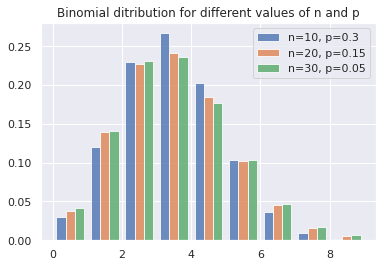
\includegraphics[width=0.5\textwidth]{../../images/binomial-distribution.png}
    \caption{Binomial distribution for different parameters $n$ and $p$.}
    \label{fig:binomial-distribution}
\end{figure}

 \item (5 marks) Exhibit the marginal posterior density for $N$, $p_1(N \mid \boldsymbol{x})$;
 
  \vspace{2ex}

\fbox{\parbox{0.92\textwidth}{
    {\bf Solution.} \lipsum[1]
}
}


\vspace{2ex}

 \item (5 marks) Return to point (a) above and consider an alternative, uninformative prior structure for $\xi$, $\pi_2$.
 Then, derive $p_2(N \mid \boldsymbol{x})$;

 \vspace{2ex}

\fbox{\parbox{0.92\textwidth}{
    {\bf Solution.} \lipsum[1]
}
}


\vspace{2ex}

 \item (10 marks) Formulate a third prior structure on $\xi$, $\pi_3$, that allows for the closed-form marginalization over the hyperparameters $\alpha$ -- see (a) -- and write out $p_3(N \mid \boldsymbol{x})$;
 
 \vspace{2ex}

    {\bf Solution.} The structure of the Geometric independent approach
    allowed the closed-form marginalization over $\nu$ and $\theta$, as expressed in
    equation \ref{eq:p1-geom-indep}. I will denote from now on $p_4$ the
    marginalized distribution of Geometric correlated approach, given by
    expression \ref{eq:p1-geom-corr}.


 \item (10 marks) Show whether each of the marginal posteriors considered is proper.
 Then, derive the posterior predictive distribution, $g_i(\tilde{x} \mid
 \boldsymbol{x})$, for each of the posteriors considered ($i = 1, 2, 3, 4$).
    
  \vspace{2ex}

\fbox{\parbox{0.92\textwidth}{
    {\bf Solution.} \lipsum[1]
}
}


\vspace{2ex}

 \item (5 marks) Consider the loss function
 \begin{equation}
 \label{eq:relative_loss}
  L(\delta(\boldsymbol{x}), N) = \left(\frac{\delta(\boldsymbol{x})-N}{N} \right)^2.
 \end{equation}
 Derive the Bayes estimator under this loss.

 \vspace{2ex}

\fbox{\parbox{0.92\textwidth}{
    {\bf Solution.} \lipsum[1]
}
}


\vspace{2ex}

\end{enumerate}

\section*{Inferring population sizes -- practice}
Consider the problem of inferring the population sizes of major herbivores~\citep{Carroll1985}.
In the first case, one is interested in estimating the number of impala (\textit{Aepyceros melampus}) herds in the Kruger National Park, in northeastern South Africa.
In an initial survey collected the following numbers of herds: $\boldsymbol{x}_{\text{impala}} = \{15, 20, 21, 23, 26\}$.
Another scientific question is the number of individual waterbuck (\textit{Kobus ellipsiprymnus}) in the same park.
The observed numbers of waterbuck in separate sightings were $\boldsymbol{x}_{\text{waterbuck}} = \{53, 57, 66, 67, 72\}$ and may be regarded (for simplicity) as independent and identically distributed.

\begin{figure}[H]
     \centering
     \begin{subfigure}[b]{0.45\textwidth}
         \centering
         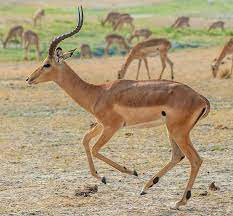
\includegraphics[scale=0.75]{figures/impala.jpeg}
         \caption{Impala}
     \end{subfigure}
     \begin{subfigure}[b]{0.45\textwidth}
         \centering
         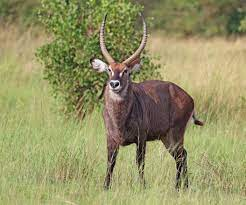
\includegraphics[scale=0.75]{figures/waterbuck.jpeg}
         \caption{Waterbuck}
     \end{subfigure}
        \caption{Two antelope species whose population sizes we want to estimate.}
        \label{fig:antelopes}
\end{figure}


\begin{enumerate}[label=\alph*)]
\setcounter{enumi}{8}
 \item (20 marks) For each data set, sketch the marginal posterior distributions $p_1(N \mid \boldsymbol{x})$, $p_2(N \mid \boldsymbol{x})$ and $p_3(N \mid \boldsymbol{x})$.
 Moreover, under each posterior,  provide (i) the Bayes estimator under quadratic loss and under the loss in (\ref{eq:relative_loss}) and (ii) a 95\% credibility interval for $N$.
 Discuss the differences and similarities between these distributions and
 estimates: do the prior modelling choices substantially impact the final
 inferences? If so, how?
 
 \vspace{2ex}

\fbox{\parbox{0.92\textwidth}{
    {\bf Solution.} \lipsum[1]
}
}


\vspace{2ex}

 \item (25 marks) Let $\bar{x} = K^{-1}\sum_{k =1}^K x_k$ and $s^2 = K^{-1}\sum_{k =1}^K (x_k-\bar{x})^2$.
 For this problem, a sample is said to be \textit{stable} if $\bar{x}/s^2 \geq (\sqrt{2} + 1)/\sqrt{2}$ and \textit{unstable} otherwise.
 Devise a simple method of moments estimator (MME) for $N$.
 Then, using a Monte Carlo simulation, compare the MME to the three Bayes estimators under quadratic loss in terms of relative mean squared error. 
 How do the Bayes estimators compare to MME in terms of the stability of the generated samples? 
 \textit{Hint}: You may want to follow the simulation setup
 of~\cite{Carroll1985}. 
 
 \vspace{2ex}

    {\bf Solution.} I first observe that both data sets are unstable by the
    above definition. The mean over variance from impala data is 1.6, while
    waterbuck's is 1.3. Both smaller than 1.71. Since the binomial
    distribution has two unknown parameters, I need to calculate two moments to
    obtain the MME. I calculate the sample mean $\hat{\mu}$ and the sample second moment $\hat{\sigma}^2 -
    \hat{\mu}^2$, where $\hat{\sigma}^2$ is the sample variance. Therefore, I build the
    following system of equations 
    \begin{gather*}
        \hat{\mu} = N\theta, \\
        \hat{\sigma}^2 = N\theta(1-\theta),
    \end{gather*} 
    that is 
    $$\hat{\sigma}^2 = \hat{\mu}(1 - \theta) \implies \hat{\theta} = 1 -
    \frac{\hat{\sigma}^2}{\hat{\mu}}$$
    and
    $$
    \hat{N} = \frac{\hat{\mu}}{\hat{\theta}} = \frac{\hat{\mu}^2}{\hat{\mu} - \hat{\sigma}^2}.
    $$
    For instance, the $N_{MME}$ calculated were 56.54 for the impala data set, and 271.84
    for the waterbuck.

    \ind The used setup to compare the
    estimators and to analyse the stability is from \cite[Section 3]{Carroll1985}. First, I generate eight samples
    with different parameters, and 
    calculate the four Bayes estimates, besides the moment estimator. For each
    sample, I also generate a perturbed sample adding one to the largest
    value. I keep the same hyperparameters defined before except the beta
    hyperparameters of $\theta$, which I increase to 2, because the
    non-informative prior was giving low $N$ estimates. The correlation in the
    last model was increased to 0.8, given the figure
    \ref{fig:binomial-distribution}. 
    
    \ind Table \ref{tab:simulations-estimates}
    presents the results. The first thing we observe is that small values of
    $\theta$ induces smaller estimates of $N$, therefore it is important to
    put stronger priors of $\theta$. This can be done studying this parameter
    in controlled spaces, where it is possible to know the population size.
    The correlated model increases the estimates, without the need of improper
    priors. THe moment estimator is undefined in some cases anf more unstable,
    but not always. 
    
\begin{table}[!ht]
    \centering
    \begin{tabular}{|c|c|c|c|c|c|c|c|c|}
        \hline
        \textbf{}          & \multicolumn{3}{c|}{\textbf{Parameters}} & \multicolumn{5}{c|}{\textbf{Estimators}}                                                 \\ \hline
        \textbf{Sample}    & \textbf{N}   & \textbf{p}  & \textbf{K}  & \textbf{Raft} & \textbf{Uninf} & \textbf{Geom id} & \textbf{Geom corr} & \textbf{Moment} \\ \hline
        \textbf{1}         & 75           & 0.32        & 5           & 45.32         & 58.99          & 50.88            & 68.52              & 78.87           \\ \hline
        \textbf{Perturbed} & 75           & 0.32        & 5           & 47.39         & 63.81          & 53.48            & 72.18              & 105.63          \\ \hline
        \textbf{2}         & 34           & 0.57        & 4           & 29.05         & 31.57          & 31.07            & 40.95              & 24.18           \\ \hline
        \textbf{Perturbed} & 34           & 0.57        & 4           & 31.11         & 35.04          & 33.35            & 43.81              & 26.16           \\ \hline
        \textbf{3}         & 37           & 0.17        & 20          & 22.28         & 27.47          & 20.92            & 27.21              & \textless 0     \\ \hline
        \textbf{Perturbed} & 37           & 0.17        & 20          & 24.28         & 30.60          & 22.61            & 29.68              & \textless{}0    \\ \hline
        \textbf{4}         & 48           & 0.06        & 15          & 9.09          & 10.62          & 8.31             & 10.49              & \textless{}0    \\ \hline
        \textbf{Perturbed} & 48           & 0.06        & 15          & 10.64         & 12.44          & 9.71             & 12.44              & \textless{}0    \\ \hline
        \textbf{5}         & 40           & 0.17        & 12          & 16.37         & 18.98          & 15.86            & 19.51              & 31.39           \\ \hline
        \textbf{Perturbed} & 40           & 0.17        & 12          & 18.34         & 21.13          & 17.50            & 21.70              & 61.12           \\ \hline
        6                  & 74           & 0.68        & 12          & 59.98         & 62.13          & 63.35            & 75.51              & 58.26           \\ \hline
        \textbf{Perturbed} & 74           & 0.68        & 12          & 61.33         & 64.08          & 65.02            & 77.28              & 59.17           \\ \hline
        \textbf{7}         & 55           & 0.48        & 20          & 42.51         & 47.14          & 45.57            & 52.93              & 42.78           \\ \hline
        \textbf{Perturbed} & 55           & 0.48        & 20          & 44.01         & 49.64          & 47.53            & 55.49              & 44.48           \\ \hline
        \textbf{8}         & 60           & 0.24        & 15          & 29.56         & 35.31          & 30.65            & 37.88              & 37.33           \\ \hline
        \textbf{Perturbed} & 60           & 0.24        & 15          & 31.46         & 37.97          & 32.72            & 40.81              & 42.84           \\ \hline
        \end{tabular}
    \caption{Simulations generated by the parameters $N, \theta$, and $K$, and the estimators calculated by each model, besides the moment estimator. For each sample, the first line indicates the estimates for it, while the second line the estimates fot the perturbed sample, adding one to the largest value.}
    \label{tab:simulations-estimates}
\end{table}
    
    \ind After that, $3 \le K \le 22$, $0 < \theta < 1$, and $1 \le N \le 100$ was
    randomly and uniformly chosen. There were 2000 generated cases with these
    parameters, and we separated them between stable, when $\hat{\mu} \ge (1 +
    1/\sqrt{2})\hat{\sigma}^2$ and unstable otherwise. We calculated the Bayes
    estimates and the moment estimate for each to obtain a Monte Carlo loss
    estimation. The results can be found in table XXX. Several samples had
    convergence problems (less than 1\%), specially in the uninformative case.
    I could not spend more time trying to solve this, because it was already
    too computationally expensive. Few simulations had serious convergence 
    problems (around 50\%), and were discarded. 

\end{enumerate}

\appendix
\section*{Appendix}
\renewcommand{\thesubsection}{\Alph{subsection}}

\subsection{Binomial and Poisson}
\label{sec:binomial-poisson}

Suppose $X|N \sim \Bin(N, p)$ and $N \sim \Poi(\mu)$. We shall derive the
distribution of $X$. By the Law of total probability, 
\begin{equation}
    \begin{split}
        \pr(X = k) &= \sum_{n=0}^{\infty} \pr(X = k|N = n)\pr(N = n) ~~~ [\pr(X = k| N = n) = 0 \text{ if } k > n] \\  
        &= \sum_{n=k}^{\infty} \binom{n}{k}p^k(1-p)^{n-k}\frac{e^{-\mu}\mu^n}{n!} \\
        &= \frac{e^{-\mu}p^k}{k!}\sum_{n=k}^{\infty} \frac{(1-p)^{n-k}}{(n-k)!}\mu^{n-k}\mu^k \\
        &= \frac{e^{-\mu}(p\mu)^k}{k!}\sum_{n=k}^{\infty} \frac{((1-p)\mu)^{n-k}}{(n-k)!} \\
        &= \frac{e^{-\mu}(p\mu)^k}{k!}\sum_{m=0}^{\infty} \frac{((1-p)\mu)^{m}}{m!} ~~~~~~~~~~~ [m = n-k] \\
        &= \frac{e^{-\mu}(p\mu)^k}{k!}e^{(1-p)\mu} \\
        &= \frac{e^{-p\mu}(p\mu)^k}{k!}, 
    \end{split}
\end{equation}
what implies $X \sim \Poi(p\cdot\mu)$.

\subsection{Prior predictive checking}
\label{sec:prior-predictive-checking}




\bibliographystyle{apalike}
\bibliography{a2}
\end{document}          
